% Options for packages loaded elsewhere
\PassOptionsToPackage{unicode}{hyperref}
\PassOptionsToPackage{hyphens}{url}
%
\documentclass[
  12pt,
]{article}
\usepackage{amsmath,amssymb}
\usepackage{iftex}
\ifPDFTeX
  \usepackage[T1]{fontenc}
  \usepackage[utf8]{inputenc}
  \usepackage{textcomp} % provide euro and other symbols
\else % if luatex or xetex
  \usepackage{unicode-math} % this also loads fontspec
  \defaultfontfeatures{Scale=MatchLowercase}
  \defaultfontfeatures[\rmfamily]{Ligatures=TeX,Scale=1}
\fi
\usepackage{lmodern}
\ifPDFTeX\else
  % xetex/luatex font selection
    \setmainfont[]{Times New Roman}
\fi
% Use upquote if available, for straight quotes in verbatim environments
\IfFileExists{upquote.sty}{\usepackage{upquote}}{}
\IfFileExists{microtype.sty}{% use microtype if available
  \usepackage[]{microtype}
  \UseMicrotypeSet[protrusion]{basicmath} % disable protrusion for tt fonts
}{}
\makeatletter
\@ifundefined{KOMAClassName}{% if non-KOMA class
  \IfFileExists{parskip.sty}{%
    \usepackage{parskip}
  }{% else
    \setlength{\parindent}{0pt}
    \setlength{\parskip}{6pt plus 2pt minus 1pt}}
}{% if KOMA class
  \KOMAoptions{parskip=half}}
\makeatother
\usepackage{xcolor}
\usepackage[margin=1in]{geometry}
\usepackage{color}
\usepackage{fancyvrb}
\newcommand{\VerbBar}{|}
\newcommand{\VERB}{\Verb[commandchars=\\\{\}]}
\DefineVerbatimEnvironment{Highlighting}{Verbatim}{commandchars=\\\{\}}
% Add ',fontsize=\small' for more characters per line
\usepackage{framed}
\definecolor{shadecolor}{RGB}{248,248,248}
\newenvironment{Shaded}{\begin{snugshade}}{\end{snugshade}}
\newcommand{\AlertTok}[1]{\textcolor[rgb]{0.94,0.16,0.16}{#1}}
\newcommand{\AnnotationTok}[1]{\textcolor[rgb]{0.56,0.35,0.01}{\textbf{\textit{#1}}}}
\newcommand{\AttributeTok}[1]{\textcolor[rgb]{0.13,0.29,0.53}{#1}}
\newcommand{\BaseNTok}[1]{\textcolor[rgb]{0.00,0.00,0.81}{#1}}
\newcommand{\BuiltInTok}[1]{#1}
\newcommand{\CharTok}[1]{\textcolor[rgb]{0.31,0.60,0.02}{#1}}
\newcommand{\CommentTok}[1]{\textcolor[rgb]{0.56,0.35,0.01}{\textit{#1}}}
\newcommand{\CommentVarTok}[1]{\textcolor[rgb]{0.56,0.35,0.01}{\textbf{\textit{#1}}}}
\newcommand{\ConstantTok}[1]{\textcolor[rgb]{0.56,0.35,0.01}{#1}}
\newcommand{\ControlFlowTok}[1]{\textcolor[rgb]{0.13,0.29,0.53}{\textbf{#1}}}
\newcommand{\DataTypeTok}[1]{\textcolor[rgb]{0.13,0.29,0.53}{#1}}
\newcommand{\DecValTok}[1]{\textcolor[rgb]{0.00,0.00,0.81}{#1}}
\newcommand{\DocumentationTok}[1]{\textcolor[rgb]{0.56,0.35,0.01}{\textbf{\textit{#1}}}}
\newcommand{\ErrorTok}[1]{\textcolor[rgb]{0.64,0.00,0.00}{\textbf{#1}}}
\newcommand{\ExtensionTok}[1]{#1}
\newcommand{\FloatTok}[1]{\textcolor[rgb]{0.00,0.00,0.81}{#1}}
\newcommand{\FunctionTok}[1]{\textcolor[rgb]{0.13,0.29,0.53}{\textbf{#1}}}
\newcommand{\ImportTok}[1]{#1}
\newcommand{\InformationTok}[1]{\textcolor[rgb]{0.56,0.35,0.01}{\textbf{\textit{#1}}}}
\newcommand{\KeywordTok}[1]{\textcolor[rgb]{0.13,0.29,0.53}{\textbf{#1}}}
\newcommand{\NormalTok}[1]{#1}
\newcommand{\OperatorTok}[1]{\textcolor[rgb]{0.81,0.36,0.00}{\textbf{#1}}}
\newcommand{\OtherTok}[1]{\textcolor[rgb]{0.56,0.35,0.01}{#1}}
\newcommand{\PreprocessorTok}[1]{\textcolor[rgb]{0.56,0.35,0.01}{\textit{#1}}}
\newcommand{\RegionMarkerTok}[1]{#1}
\newcommand{\SpecialCharTok}[1]{\textcolor[rgb]{0.81,0.36,0.00}{\textbf{#1}}}
\newcommand{\SpecialStringTok}[1]{\textcolor[rgb]{0.31,0.60,0.02}{#1}}
\newcommand{\StringTok}[1]{\textcolor[rgb]{0.31,0.60,0.02}{#1}}
\newcommand{\VariableTok}[1]{\textcolor[rgb]{0.00,0.00,0.00}{#1}}
\newcommand{\VerbatimStringTok}[1]{\textcolor[rgb]{0.31,0.60,0.02}{#1}}
\newcommand{\WarningTok}[1]{\textcolor[rgb]{0.56,0.35,0.01}{\textbf{\textit{#1}}}}
\usepackage{longtable,booktabs,array}
\usepackage{calc} % for calculating minipage widths
% Correct order of tables after \paragraph or \subparagraph
\usepackage{etoolbox}
\makeatletter
\patchcmd\longtable{\par}{\if@noskipsec\mbox{}\fi\par}{}{}
\makeatother
% Allow footnotes in longtable head/foot
\IfFileExists{footnotehyper.sty}{\usepackage{footnotehyper}}{\usepackage{footnote}}
\makesavenoteenv{longtable}
\usepackage{graphicx}
\makeatletter
\def\maxwidth{\ifdim\Gin@nat@width>\linewidth\linewidth\else\Gin@nat@width\fi}
\def\maxheight{\ifdim\Gin@nat@height>\textheight\textheight\else\Gin@nat@height\fi}
\makeatother
% Scale images if necessary, so that they will not overflow the page
% margins by default, and it is still possible to overwrite the defaults
% using explicit options in \includegraphics[width, height, ...]{}
\setkeys{Gin}{width=\maxwidth,height=\maxheight,keepaspectratio}
% Set default figure placement to htbp
\makeatletter
\def\fps@figure{htbp}
\makeatother
\setlength{\emergencystretch}{3em} % prevent overfull lines
\providecommand{\tightlist}{%
  \setlength{\itemsep}{0pt}\setlength{\parskip}{0pt}}
\setcounter{secnumdepth}{5}
% definitions for citeproc citations
\NewDocumentCommand\citeproctext{}{}
\NewDocumentCommand\citeproc{mm}{%
  \begingroup\def\citeproctext{#2}\cite{#1}\endgroup}
\makeatletter
 % allow citations to break across lines
 \let\@cite@ofmt\@firstofone
 % avoid brackets around text for \cite:
 \def\@biblabel#1{}
 \def\@cite#1#2{{#1\if@tempswa , #2\fi}}
\makeatother
\newlength{\cslhangindent}
\setlength{\cslhangindent}{1.5em}
\newlength{\csllabelwidth}
\setlength{\csllabelwidth}{3em}
\newenvironment{CSLReferences}[2] % #1 hanging-indent, #2 entry-spacing
 {\begin{list}{}{%
  \setlength{\itemindent}{0pt}
  \setlength{\leftmargin}{0pt}
  \setlength{\parsep}{0pt}
  % turn on hanging indent if param 1 is 1
  \ifodd #1
   \setlength{\leftmargin}{\cslhangindent}
   \setlength{\itemindent}{-1\cslhangindent}
  \fi
  % set entry spacing
  \setlength{\itemsep}{#2\baselineskip}}}
 {\end{list}}
\usepackage{calc}
\newcommand{\CSLBlock}[1]{\hfill\break\parbox[t]{\linewidth}{\strut\ignorespaces#1\strut}}
\newcommand{\CSLLeftMargin}[1]{\parbox[t]{\csllabelwidth}{\strut#1\strut}}
\newcommand{\CSLRightInline}[1]{\parbox[t]{\linewidth - \csllabelwidth}{\strut#1\strut}}
\newcommand{\CSLIndent}[1]{\hspace{\cslhangindent}#1}
\usepackage{tcolorbox}
\usepackage{amssymb}
\usepackage{yfonts}
\usepackage{bm}
\usepackage{titlesec}
\usepackage{kbordermatrix}


\newtcolorbox{greybox}{
  colback=white,
  colframe=blue,
  coltext=black,
  boxsep=5pt,
  arc=4pt}
  
\newcommand{\sectionbreak}{\clearpage}

 
\newcommand{\ds}[4]{\sum_{{#1}=1}^{#3}\sum_{{#2}=1}^{#4}}
\newcommand{\us}[3]{\mathop{\sum\sum}_{1\leq{#2}<{#1}\leq{#3}}}

\newcommand{\ol}[1]{\overline{#1}}
\newcommand{\ul}[1]{\underline{#1}}

\newcommand{\amin}[1]{\mathop{\text{argmin}}_{#1}}
\newcommand{\amax}[1]{\mathop{\text{argmax}}_{#1}}

\newcommand{\ci}{\perp\!\!\!\perp}

\newcommand{\mc}[1]{\mathcal{#1}}
\newcommand{\mb}[1]{\mathbb{#1}}
\newcommand{\mf}[1]{\mathfrak{#1}}

\newcommand{\eps}{\epsilon}
\newcommand{\lbd}{\lambda}
\newcommand{\alp}{\alpha}
\newcommand{\df}{=:}
\newcommand{\am}[1]{\mathop{\text{argmin}}_{#1}}
\newcommand{\ls}[2]{\mathop{\sum\sum}_{#1}^{#2}}
\newcommand{\ijs}{\mathop{\sum\sum}_{1\leq i<j\leq n}}
\newcommand{\jis}{\mathop{\sum\sum}_{1\leq j<i\leq n}}
\newcommand{\sij}{\sum_{i=1}^n\sum_{j=1}^n}
	
\ifLuaTeX
  \usepackage{selnolig}  % disable illegal ligatures
\fi
\usepackage{bookmark}
\IfFileExists{xurl.sty}{\usepackage{xurl}}{} % add URL line breaks if available
\urlstyle{same}
\hypersetup{
  pdfauthor={Jan de Leeuw - University of California Los Angeles},
  hidelinks,
  pdfcreator={LaTeX via pandoc}}

\title{Smacof at 50: A Manual\\
Part 2: Non-metric Smacof}
\author{Jan de Leeuw - University of California Los Angeles}
\date{Started March 30 2024, Version of April 07, 2024}

\begin{document}
\maketitle
\begin{abstract}
TBD
\end{abstract}

{
\setcounter{tocdepth}{4}
\tableofcontents
}
\textbf{Note:} This is a working manuscript which will be expanded/updated
frequently. All suggestions for improvement are welcome. All Rmd, tex,
html, pdf, R, and C files are in the public domain. Attribution will be
appreciated, but is not required. The code files can be found at
\url{https://github.com/deleeuw/smacofCode}, the manual files at
\url{https://github.com/deleeuw/smacofManual}, and the example files
at \url{https://github.com/deleeuw/smacofExamples}.

\sectionbreak

\section{Introduction}\label{introduction}

pick and rank

\section{Loss Function}\label{loss-function}

\[
\sigma(X,\Delta_1,\cdots,\Delta_s)=\frac{\sum_{r=1}^s\sum_{i,j} w_{ijr}(\delta_{ijr}-d_{ij}(X))^2}{\sum_{r=1}^s\sum_{i,j} w_{ijr}d_{ij}^2(X))}
\]
which must be minimized over \(X\) and over \(\delta_r\in\mathcal{K}_r\), with \(\mathcal{K}_r\) pointed polyhedral convex cones, defined by a partial order
\(\leq_r\).

Minimize of \(X\) for given \(\delta_{ijr}\).
\[
\sigma_R(X,\Delta_1,\cdots,\Delta_s)=\sum_{r=1}^s\sum_{i,j} w_{ijr}\delta_{ijr}^2-2\sum_{r=1}^s\sum_{i,j} w_{ijr}\delta_{ijr}d_{ij}(X)+\sum_{r=1}^s\sum_{i,j} w_{ijr}d_{ij}^2(X))
\]
Nor use the basic smacof inequality
\[
d_{ij}(X)\geq\frac{1}{d_{ij}(Y)}\text{tr}\ X'A_{ij}Y 
\]
so that
\[
\sum_{r=1}^s\sum_{i,j} w_{ijr}\delta_{ijr}d_{ij}(X)\geq
\text{tr}\ X'B(Y)Y
\]
\[
B(Y):=\sum_{r=1}^s\sum_{i,j} w_{ijr}\frac{\delta_{ijr}}{d_{ij}(Y)}A_{ij}
\]
Also
\[
V:=\sum_{r=1}^s\sum_{i,j} w_{ijr}A_{ij}
\]
So that
\[
\sigma_R(X)\leq K-2\text{tr}\ X'B(Y)Y+\text{tr}\ X'VX
\]
and the smacof update over \(X\) with \(\text{tr}\ X'VX=1\) is the same
as in smacofRR.

\section{Paired Comparisons}\label{paired-comparisons}

THe paired comparison method of data collection is the simplest and
the most basic one of the Cartwheel methods.

Positive Orthant / Absolute Value / Pairwise

De Leeuw (1970)
De Leeuw (2018)
Hartmann (1979)
Guttman (1969)
Johnson (1973)

Suppose datum \(r\) says that that \((i,j)<(k,l)\). Then \(w_{ijr}\) and \(w_{klr}\)
are non-zero and all other elements of \(W_r\) are zero.
Thus
\[
w_{ijr}(\delta_{ijr}-d_{ij})^2+w_{klr}(\delta_{klr}-d_{kl})^2
\]
Must be minimized over \(\delta_{ijr}\leq\delta_{klr}\). If \(d_{ij}\leq d_{kl}\)
then \(\hat d_{ijr}=d_{ij}\) and \(\hat d_{klr}=d_{kl}\), and otherwise
\[
\hat d_{ijr}=\hat d_{klr}=\frac{w_{ijr}d_{ij}+w_{klr}d_{kl}}{w_{ijr}+w_{klr}}
\]
Thus

\[w_{ijr}(\hat d_{ijr}-d_{ij})^2+w_{klr}(\hat d_{klr}-d_{kl})^2\]
is zero if the order of \(d_{ij}\) and \(d_{kl}\) is the same as the order in the data
and

\[
\frac{w_{ijr}w_{klr}}{w_{ijr}+w_{klr}}(d_{ij}-d_{kl})^2
\]

So far we have only considered the forced-choice situation in which
the subject has to choose one of the pairs. If we allow for the alternative
that \((i,j)\) and \((k,l)\) are equally similar then we can choose between two approaches. In the \emph{primary approach} we incur no loss for this pair, no matter what \(d_{ij}(X)\) and \(d_{kl}(X)\) are. In the \emph{secondary approach} we require that \(\delta_{ijr}=\delta_{klr}\) and consequently we add to the loss if
\(d_{ij}X)\not= d_{kl}(X)\).

\section{Triads}\label{triads}

We have implemented three different versions of the method of triads, in which stimuli are presented three at a time,
at the corners of an equilateral triangle, as in
\ldots{}

In the first one we present all
\(\binom{n}{3}=\frac16 n(n-1)(n-2)\approx\frac16n^3\)
triples of stimuli and we ask the subject to rank the
three similarities between them. More precisely we ask for the two pairs with the largest and smallest similarity,
and we interpret the responses as giving us a rank order.
Coombs (1954) calls this the \emph{method of similarities},
and Torgerson (1958) calls it the \emph{complete method of triads}.

The second method was first proposed by Richardson (1938),
as the \emph{method of triadic cobinations}. Every triad is presented three times using a slightly different layout.
\ldots{}
We ask the subject which one of the top stimuli is most similar to the bottom stimulus. This requires
\(n\binom{n-1}{2}=\frac12n(n-1)(n-2)\approx\frac12n^3\)
presentations for a complete set. Since there is only
one comparision involved, this is a special case of
the paired comparisons method, in which the pairs always
have excetly one stimulus in common. Coombs (1954) call this the \emph{method of propellors} because we only draw lines
from the bottom stimulus (the ``hub'') to the two stimuli
at the top.

\section{Richardson Hub Method}\label{richardson-hub-method}

each triple presented three times, with a different hub each time
which one of the two is maximally similar to the hub stimulus. Thus the data
is the single inequality \((i,k) < (j,k)\). Coombs calls this the \ldots{}

\section{Conditional Rank Orders -- Klingberg}\label{conditional-rank-orders-klingberg}

\section{Full Rank Orders}\label{full-rank-orders}

\section{A Paired Comparison Example}\label{a-paired-comparison-example}

The objects that we want to scale are 10 Dutch political parties.

\begin{Shaded}
\begin{Highlighting}[]
\NormalTok{parties}
\end{Highlighting}
\end{Shaded}

\begin{verbatim}
##  [1] "GL"   "PvdA" "VVD"  "D66"  "CDA"  "SP"   "PvdD" "CU"   "FVD"  "SGP"
\end{verbatim}

There is only one subject, and it is me. I used the program \texttt{smacofMakeRandomPairs()} to generate
and present to me 50 random pairs of pairs \((i,j)\) and \((k,l)\). One such pair looks like

\begin{center}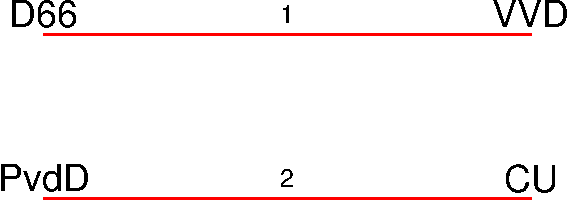
\includegraphics{smacofNM_files/figure-latex/apair-1} \end{center}

\begin{verbatim}
## (D66,VVD) and (PvdD,CU)
## most similar pair:
\end{verbatim}

In Rstudio the graphics are in the plot window, the text is in the console. If
you run R from the terminal the text will be in the terminal, and the graphics will
be in the R graphics device for the session.

It took me about
5 minutes to make the 50 binary choices, duly recorded by the program. I left The Netherlands almost 40 years ago, so I am far from an expert on Dutch politics, so
my choices may be far off the mark.

The data, with the four indices first and then the choice, are

\begin{verbatim}
##     i  j  k  l  
## 1   8  5  2  9 1
## 2   4  1  1  2 2
## 3   1  3  2  7 2
## 4   5  2  2  7 2
## 5   2  9  9  8 2
## 6   7  5  9 10 1
## 7   1 10 10  8 2
## 8   9 10  9  4 2
## 9   5  2  5  9 2
## 10  4  1 10  7 1
## 11  1  3  5 10 2
## 12  4 10  1 10 1
## 13  5  4  8  5 2
## 14  5  1  4  2 2
## 15  4 10  5  2 2
## 16  1  3  9 10 2
## 17  4  7  4  3 2
## 18  4  1 10  7 1
## 19  6  4  5  4 2
## 20  6  1  9  3 2
## 21  8  3  4  3 1
## 22 10  7  6  1 2
## 23  4  1  9  8 1
## 24 10  7  2  6 2
## 25  8  6  5  4 2
## 26  8  7  4  1 2
## 27  6  7  1  2 2
## 28  9  7  4  3 2
## 29  4  8  6  4 1
## 30  2  7  9  7 1
## 31  2  8  9  4 1
## 32  4  7  6  4 1
## 33  5  9  9 10 1
## 34  1  8  4  2 2
## 35  1  3  9  7 1
## 36 10  8  3  6 1
## 37  1  3  6  7 1
## 38  1 10  9  8 2
## 39  1  2 10  2 1
## 40  2  9  9  8 2
## 41  6 10  9  4 2
## 42 10  2  6  5 2
## 43  1  7  7  5 1
## 44  3  5 10  8 1
## 45  5  9  2  8 1
## 46  9  8  9 10 1
## 47  9  8  6  4 1
## 48  9  4  6  1 1
## 49  2  8  4  7 2
## 50  4  1  9  4 1
\end{verbatim}

Thus in the first row I say that the pair \((8,5)\) is more similar than \((2,9)\), in other words (CU, CDA) is more similar than (PvdA, FVD).

In order to start the iterative process we need an initial configuration. Insipred by De Gruijter (1967) I used
the infamous left-right horseshoe.

\begin{center}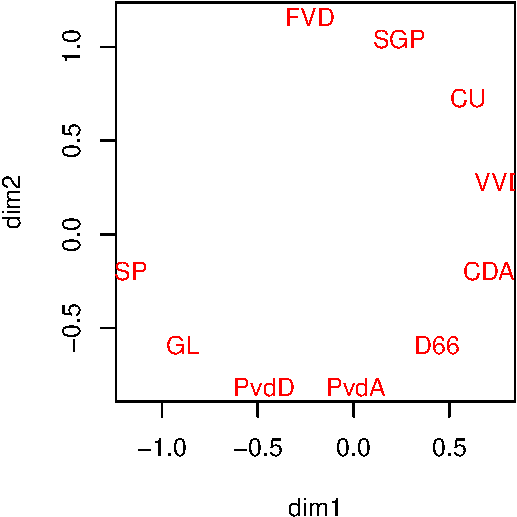
\includegraphics{smacofNM_files/figure-latex/partiesxold-1} \end{center}

\begin{Shaded}
\begin{Highlighting}[]
\FunctionTok{source}\NormalTok{(}\StringTok{"../../smacofCode/smacofNM/smacofNMforPairs.R"}\NormalTok{)}
\NormalTok{partiesResult }\OtherTok{\textless{}{-}} \FunctionTok{smacofNMforPairs}\NormalTok{(partiesData, partiesXold, }
                                  \AttributeTok{eps =} \FloatTok{1e{-}15}\NormalTok{, }\AttributeTok{itmax =} \DecValTok{1000}\NormalTok{, }\AttributeTok{verbose =} \ConstantTok{FALSE}\NormalTok{)}
\end{Highlighting}
\end{Shaded}

We have nice smooth monotone convergence. The convergence criterion is reached
in 344 iterations and the stress is \ensuremath{1.3573576\times 10^{-14}}, i.e.
practically zero. Thus we have actually found a solution to the system of
50 nonlinear inequalities defined by the data. This means two things. In the
first place I am consistent in my choices, and in the second place the solution
is undoubtedly far from unique. The map is

\begin{center}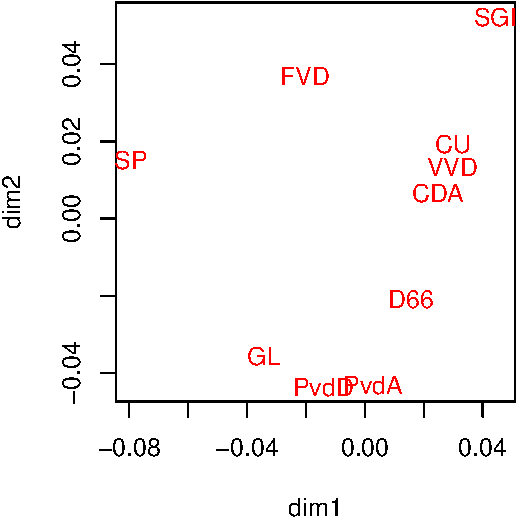
\includegraphics{smacofNM_files/figure-latex/partiesxnew-1} \end{center}

We are still reasonably close to the horseshoe, showing the influence of the
initial configuration. Of course the main reason for the non-uniqueness is
not the consistency of my choices, but the fact that we have used only 50
pairs from the \texttt{choose(choose(10,\ 2),\ 2)} = 990 possible
ones. The solution will become much tighter if there are more pairs, either
from a single subject, or from a number of subjects (in which case we would
certainly prefer MDS with parameters for individual differences).

\section{A Rank Order Example}\label{a-rank-order-example}

\begin{Shaded}
\begin{Highlighting}[]
\FunctionTok{library}\NormalTok{(MASS)}

\FunctionTok{source}\NormalTok{(}\StringTok{"../../smacofCode/smacofNM/smacofConvert.R"}\NormalTok{)}
\FunctionTok{source}\NormalTok{(}\StringTok{"../../smacofCode/smacofNM/smacofMakeData.R"}\NormalTok{)}
\FunctionTok{source}\NormalTok{(}\StringTok{"../../smacofCode/smacofNM/smacofMonotoneRegression.R"}\NormalTok{)}
\FunctionTok{source}\NormalTok{(}\StringTok{"../../smacofCode/smacofNM/smacofPlots.R"}\NormalTok{)}

\FunctionTok{data}\NormalTok{(ekman, }\AttributeTok{package =} \StringTok{"smacof"}\NormalTok{)}
\NormalTok{ekman }\OtherTok{\textless{}{-}} \DecValTok{1} \SpecialCharTok{{-}}\NormalTok{ ekman }
\NormalTok{ekmanData }\OtherTok{\textless{}{-}} \FunctionTok{smacofMakeRankOrderData}\NormalTok{(ekman)}
\NormalTok{ekmanXold }\OtherTok{\textless{}{-}} \FunctionTok{matrix}\NormalTok{(}\FunctionTok{c}\NormalTok{(}\SpecialCharTok{{-}}\FloatTok{0.1576320}\NormalTok{, }\SpecialCharTok{{-}}\FloatTok{0.54429773}\NormalTok{,}
                      \SpecialCharTok{{-}}\FloatTok{0.2169837}\NormalTok{, }\SpecialCharTok{{-}}\FloatTok{0.50815312}\NormalTok{,}
                      \SpecialCharTok{{-}}\FloatTok{0.4778581}\NormalTok{, }\SpecialCharTok{{-}}\FloatTok{0.31203061}\NormalTok{,}
                      \SpecialCharTok{{-}}\FloatTok{0.5131424}\NormalTok{, }\SpecialCharTok{{-}}\FloatTok{0.23393512}\NormalTok{,}
                      \SpecialCharTok{{-}}\FloatTok{0.5338027}\NormalTok{,  }\FloatTok{0.09175252}\NormalTok{,}
                      \SpecialCharTok{{-}}\FloatTok{0.4368053}\NormalTok{,  }\FloatTok{0.36071649}\NormalTok{,}
                      \SpecialCharTok{{-}}\FloatTok{0.2650675}\NormalTok{,  }\FloatTok{0.52174944}\NormalTok{,}
                      \SpecialCharTok{{-}}\FloatTok{0.1374662}\NormalTok{, }\FloatTok{0.57443857}\NormalTok{,}
                      \FloatTok{0.3162169}\NormalTok{,  }\FloatTok{0.46015778}\NormalTok{,}
                      \FloatTok{0.4575480}\NormalTok{,  }\FloatTok{0.24454905}\NormalTok{,}
                      \FloatTok{0.5210238}\NormalTok{,  }\FloatTok{0.03357499}\NormalTok{,}
                      \FloatTok{0.5128727}\NormalTok{, }\SpecialCharTok{{-}}\FloatTok{0.13074190}\NormalTok{,}
                      \FloatTok{0.4824539}\NormalTok{, }\SpecialCharTok{{-}}\FloatTok{0.22250509}\NormalTok{,}
                      \FloatTok{0.4486425}\NormalTok{, }\SpecialCharTok{{-}}\FloatTok{0.33527525}\NormalTok{), }\DecValTok{14}\NormalTok{, }\DecValTok{2}\NormalTok{, }\AttributeTok{byrow =} \ConstantTok{TRUE}\NormalTok{)}
\end{Highlighting}
\end{Shaded}

\section{Code}\label{code}

\subsection{Make the cartwheels and ask for choices}\label{make-the-cartwheels-and-ask-for-choices}

\begin{Shaded}
\begin{Highlighting}[]
\NormalTok{smacofMakeAllTriads }\OtherTok{\textless{}{-}} \ControlFlowTok{function}\NormalTok{(names, }\AttributeTok{complete =} \ConstantTok{TRUE}\NormalTok{) \{}
\NormalTok{  outfile }\OtherTok{\textless{}{-}} \FunctionTok{file}\NormalTok{(}\StringTok{"./output.txt"}\NormalTok{, }\AttributeTok{open =} \StringTok{"w"}\NormalTok{)}
\NormalTok{  n }\OtherTok{\textless{}{-}} \FunctionTok{length}\NormalTok{(names)}
\NormalTok{  m }\OtherTok{\textless{}{-}} \FunctionTok{choose}\NormalTok{(n, }\DecValTok{3}\NormalTok{)}
\NormalTok{  z }\OtherTok{\textless{}{-}} \FunctionTok{t}\NormalTok{(}\FunctionTok{combn}\NormalTok{(n, }\DecValTok{3}\NormalTok{))[}\FunctionTok{sample}\NormalTok{(}\DecValTok{1}\SpecialCharTok{:}\NormalTok{m, m), ]}
\NormalTok{  z }\OtherTok{\textless{}{-}} \FunctionTok{t}\NormalTok{(}\FunctionTok{apply}\NormalTok{(z, }\DecValTok{1}\NormalTok{, }\ControlFlowTok{function}\NormalTok{(x)}
    \FunctionTok{sample}\NormalTok{(x, }\FunctionTok{length}\NormalTok{(x))))}
\NormalTok{  y }\OtherTok{\textless{}{-}} \DecValTok{8} \SpecialCharTok{{-}} \DecValTok{3} \SpecialCharTok{*} \FunctionTok{sqrt}\NormalTok{(}\DecValTok{3}\NormalTok{)}
  \ControlFlowTok{for}\NormalTok{ (i }\ControlFlowTok{in} \DecValTok{1}\SpecialCharTok{:}\NormalTok{m) \{}
\NormalTok{    x }\OtherTok{\textless{}{-}}\NormalTok{ z[i, ]}
    \FunctionTok{plot}\NormalTok{(}
      \DecValTok{1}\SpecialCharTok{:}\DecValTok{10}\NormalTok{,}
      \AttributeTok{axes =} \ConstantTok{FALSE}\NormalTok{,}
      \AttributeTok{type =} \StringTok{"n"}\NormalTok{,}
      \AttributeTok{xlab =} \StringTok{""}\NormalTok{,}
      \AttributeTok{ylab =} \StringTok{""}
\NormalTok{    )}
    \FunctionTok{lines}\NormalTok{(}\FunctionTok{c}\NormalTok{(}\DecValTok{2}\NormalTok{, }\DecValTok{8}\NormalTok{), }\FunctionTok{c}\NormalTok{(}\DecValTok{8}\NormalTok{, }\DecValTok{8}\NormalTok{), }\AttributeTok{col =} \StringTok{"RED"}\NormalTok{)}
    \FunctionTok{lines}\NormalTok{(}\FunctionTok{c}\NormalTok{(}\DecValTok{2}\NormalTok{, }\DecValTok{5}\NormalTok{), }\FunctionTok{c}\NormalTok{(}\DecValTok{8}\NormalTok{, y), }\AttributeTok{col =} \StringTok{"RED"}\NormalTok{)}
    \FunctionTok{lines}\NormalTok{(}\FunctionTok{c}\NormalTok{(}\DecValTok{8}\NormalTok{, }\DecValTok{5}\NormalTok{), }\FunctionTok{c}\NormalTok{(}\DecValTok{8}\NormalTok{, y), }\AttributeTok{col =} \StringTok{"RED"}\NormalTok{)}
    \FunctionTok{text}\NormalTok{(}\FunctionTok{c}\NormalTok{(}\DecValTok{2}\NormalTok{, }\DecValTok{8}\NormalTok{, }\DecValTok{5}\NormalTok{), }\FunctionTok{c}\NormalTok{(}\FloatTok{8.2}\NormalTok{, }\FloatTok{8.2}\NormalTok{, y }\SpecialCharTok{{-}}\NormalTok{ .}\DecValTok{2}\NormalTok{),}
         \FunctionTok{c}\NormalTok{(names[x[}\DecValTok{1}\NormalTok{]], names[x[}\DecValTok{2}\NormalTok{]], names[x[}\DecValTok{3}\NormalTok{]]), }\AttributeTok{cex =} \FloatTok{1.5}\NormalTok{)}
    \FunctionTok{text}\NormalTok{(}\DecValTok{5}\NormalTok{, }\FloatTok{8.5}\NormalTok{, }\StringTok{"1"}\NormalTok{)}
    \FunctionTok{text}\NormalTok{(}\DecValTok{3}\NormalTok{, }\FloatTok{5.40}\NormalTok{, }\StringTok{"2"}\NormalTok{)}
    \FunctionTok{text}\NormalTok{(}\DecValTok{7}\NormalTok{, }\FloatTok{5.40}\NormalTok{, }\StringTok{"3"}\NormalTok{)}
    \FunctionTok{print}\NormalTok{(}\FunctionTok{c}\NormalTok{(}\FunctionTok{noquote}\NormalTok{(names[x[}\DecValTok{1}\NormalTok{]]), }\FunctionTok{noquote}\NormalTok{(names[x[}\DecValTok{2}\NormalTok{]]), }\FunctionTok{noquote}\NormalTok{(names[x[}\DecValTok{3}\NormalTok{]])))}
\NormalTok{    u }\OtherTok{\textless{}{-}} \FunctionTok{readline}\NormalTok{(}\StringTok{"most similar pair: "}\NormalTok{)}
    \ControlFlowTok{if}\NormalTok{ (complete) \{}
\NormalTok{      v }\OtherTok{\textless{}{-}} \FunctionTok{readline}\NormalTok{(}\StringTok{"least similar pair: "}\NormalTok{)}
      \FunctionTok{write}\NormalTok{(}\FunctionTok{c}\NormalTok{(x, u, v), }\AttributeTok{ncolumns =} \DecValTok{5}\NormalTok{, }\AttributeTok{file =}\NormalTok{ outfile)}
\NormalTok{    \} }\ControlFlowTok{else}\NormalTok{ \{}
      \FunctionTok{write}\NormalTok{(}\FunctionTok{c}\NormalTok{(x, u), }\AttributeTok{ncolumns =} \DecValTok{4}\NormalTok{, }\AttributeTok{file =}\NormalTok{ outfile)}
\NormalTok{    \}}
\NormalTok{  \}}
  \FunctionTok{close}\NormalTok{(outfile)}
\NormalTok{\}}

\NormalTok{smacofMakeRandomTriads }\OtherTok{\textless{}{-}}
  \ControlFlowTok{function}\NormalTok{(names, nrandom, }\AttributeTok{complete =} \ConstantTok{TRUE}\NormalTok{) \{}
\NormalTok{    outfile }\OtherTok{\textless{}{-}} \FunctionTok{file}\NormalTok{(}\StringTok{"./output.txt"}\NormalTok{, }\AttributeTok{open =} \StringTok{"w"}\NormalTok{)}
\NormalTok{    n }\OtherTok{\textless{}{-}} \FunctionTok{length}\NormalTok{(names)}
\NormalTok{    y }\OtherTok{\textless{}{-}} \DecValTok{8} \SpecialCharTok{{-}} \DecValTok{3} \SpecialCharTok{*} \FunctionTok{sqrt}\NormalTok{(}\DecValTok{3}\NormalTok{)}
    \ControlFlowTok{for}\NormalTok{ (i }\ControlFlowTok{in} \DecValTok{1}\SpecialCharTok{:}\NormalTok{nrandom) \{}
\NormalTok{      x }\OtherTok{\textless{}{-}} \FunctionTok{sample}\NormalTok{(}\DecValTok{1}\SpecialCharTok{:}\NormalTok{n, }\DecValTok{3}\NormalTok{)}
      \FunctionTok{plot}\NormalTok{(}
        \DecValTok{1}\SpecialCharTok{:}\DecValTok{10}\NormalTok{,}
        \AttributeTok{axes =} \ConstantTok{FALSE}\NormalTok{,}
        \AttributeTok{type =} \StringTok{"n"}\NormalTok{,}
        \AttributeTok{xlab =} \StringTok{""}\NormalTok{,}
        \AttributeTok{ylab =} \StringTok{""}
\NormalTok{      )}
      \FunctionTok{lines}\NormalTok{(}\FunctionTok{c}\NormalTok{(}\DecValTok{2}\NormalTok{, }\DecValTok{8}\NormalTok{), }\FunctionTok{c}\NormalTok{(}\DecValTok{8}\NormalTok{, }\DecValTok{8}\NormalTok{), }\AttributeTok{col =} \StringTok{"RED"}\NormalTok{)}
      \FunctionTok{lines}\NormalTok{(}\FunctionTok{c}\NormalTok{(}\DecValTok{2}\NormalTok{, }\DecValTok{5}\NormalTok{), }\FunctionTok{c}\NormalTok{(}\DecValTok{8}\NormalTok{, y), }\AttributeTok{col =} \StringTok{"RED"}\NormalTok{)}
      \FunctionTok{lines}\NormalTok{(}\FunctionTok{c}\NormalTok{(}\DecValTok{8}\NormalTok{, }\DecValTok{5}\NormalTok{), }\FunctionTok{c}\NormalTok{(}\DecValTok{8}\NormalTok{, y), }\AttributeTok{col =} \StringTok{"RED"}\NormalTok{)}
      \FunctionTok{text}\NormalTok{(}\FunctionTok{c}\NormalTok{(}\DecValTok{2}\NormalTok{, }\DecValTok{8}\NormalTok{, }\DecValTok{5}\NormalTok{), }\FunctionTok{c}\NormalTok{(}\FloatTok{8.2}\NormalTok{, }\FloatTok{8.2}\NormalTok{, y }\SpecialCharTok{{-}}\NormalTok{ .}\DecValTok{2}\NormalTok{),}
           \FunctionTok{c}\NormalTok{(names[x[}\DecValTok{1}\NormalTok{]], names[x[}\DecValTok{2}\NormalTok{]], names[x[}\DecValTok{3}\NormalTok{]]), }\AttributeTok{cex =} \FloatTok{1.5}\NormalTok{)}
      \FunctionTok{text}\NormalTok{(}\DecValTok{5}\NormalTok{, }\FloatTok{8.5}\NormalTok{, }\StringTok{"1"}\NormalTok{)}
      \FunctionTok{text}\NormalTok{(}\DecValTok{3}\NormalTok{, }\FloatTok{5.40}\NormalTok{, }\StringTok{"2"}\NormalTok{)}
      \FunctionTok{text}\NormalTok{(}\DecValTok{7}\NormalTok{, }\FloatTok{5.40}\NormalTok{, }\StringTok{"3"}\NormalTok{)}
      \FunctionTok{print}\NormalTok{(}\FunctionTok{c}\NormalTok{(}\FunctionTok{noquote}\NormalTok{(names[x[}\DecValTok{1}\NormalTok{]]), }\FunctionTok{noquote}\NormalTok{(names[x[}\DecValTok{2}\NormalTok{]]), }\FunctionTok{noquote}\NormalTok{(names[x[}\DecValTok{3}\NormalTok{]])))}
\NormalTok{      u }\OtherTok{\textless{}{-}} \FunctionTok{readline}\NormalTok{(}\StringTok{"most similar pair: "}\NormalTok{)}
      \ControlFlowTok{if}\NormalTok{ (complete) \{}
\NormalTok{        v }\OtherTok{\textless{}{-}} \FunctionTok{readline}\NormalTok{(}\StringTok{"least similar pair: "}\NormalTok{)}
        \FunctionTok{write}\NormalTok{(}\FunctionTok{c}\NormalTok{(x, u, v), }\AttributeTok{ncolumns =} \DecValTok{5}\NormalTok{, }\AttributeTok{file =}\NormalTok{ outfile)}
\NormalTok{      \} }\ControlFlowTok{else}\NormalTok{ \{}
        \FunctionTok{write}\NormalTok{(}\FunctionTok{c}\NormalTok{(x, u), }\AttributeTok{ncolumns =} \DecValTok{4}\NormalTok{, }\AttributeTok{file =}\NormalTok{ outfile)}
\NormalTok{      \}}
\NormalTok{    \}}
    \FunctionTok{close}\NormalTok{(outfile)}
\NormalTok{  \}}

\NormalTok{smacofMakeAllPairs }\OtherTok{\textless{}{-}} \ControlFlowTok{function}\NormalTok{(names) \{}
\NormalTok{  outfile }\OtherTok{\textless{}{-}} \FunctionTok{file}\NormalTok{(}\StringTok{"./output.txt"}\NormalTok{, }\AttributeTok{open =} \StringTok{"w"}\NormalTok{)}
\NormalTok{  n }\OtherTok{\textless{}{-}} \FunctionTok{length}\NormalTok{(names)}
\NormalTok{  l }\OtherTok{\textless{}{-}} \FunctionTok{choose}\NormalTok{(n, }\DecValTok{2}\NormalTok{)}
\NormalTok{  u }\OtherTok{\textless{}{-}} \FunctionTok{combn}\NormalTok{(n, }\DecValTok{2}\NormalTok{)}
\NormalTok{  u }\OtherTok{\textless{}{-}} \FunctionTok{apply}\NormalTok{(u, }\DecValTok{2}\NormalTok{, }\ControlFlowTok{function}\NormalTok{(x)}
    \FunctionTok{sample}\NormalTok{(x, }\FunctionTok{length}\NormalTok{(x)))}
\NormalTok{  m }\OtherTok{\textless{}{-}} \FunctionTok{choose}\NormalTok{(l, }\DecValTok{2}\NormalTok{)}
\NormalTok{  v }\OtherTok{\textless{}{-}} \FunctionTok{combn}\NormalTok{(l, }\DecValTok{2}\NormalTok{)[, }\FunctionTok{sample}\NormalTok{(}\DecValTok{1}\SpecialCharTok{:}\NormalTok{m, m)]}
\NormalTok{  v }\OtherTok{\textless{}{-}} \FunctionTok{apply}\NormalTok{(v, }\DecValTok{2}\NormalTok{, }\ControlFlowTok{function}\NormalTok{(x)}
    \FunctionTok{sample}\NormalTok{(x, }\FunctionTok{length}\NormalTok{(x)))}
  \ControlFlowTok{for}\NormalTok{ (i }\ControlFlowTok{in} \DecValTok{1}\SpecialCharTok{:}\NormalTok{m) \{}
\NormalTok{    x }\OtherTok{\textless{}{-}} \FunctionTok{c}\NormalTok{(u[, v[}\DecValTok{1}\NormalTok{, i]], u[, v[}\DecValTok{2}\NormalTok{, i]])}
    \FunctionTok{plot}\NormalTok{(}
      \DecValTok{1}\SpecialCharTok{:}\DecValTok{10}\NormalTok{,}
      \AttributeTok{axes =} \ConstantTok{FALSE}\NormalTok{,}
      \AttributeTok{type =} \StringTok{"n"}\NormalTok{,}
      \AttributeTok{xlab =} \StringTok{""}\NormalTok{,}
      \AttributeTok{ylab =} \StringTok{""}
\NormalTok{    )}
    \FunctionTok{lines}\NormalTok{(}\FunctionTok{c}\NormalTok{(}\DecValTok{2}\NormalTok{, }\DecValTok{8}\NormalTok{), }\FunctionTok{c}\NormalTok{(}\DecValTok{8}\NormalTok{, }\DecValTok{8}\NormalTok{), }\AttributeTok{col =} \StringTok{"RED"}\NormalTok{)}
    \FunctionTok{lines}\NormalTok{(}\FunctionTok{c}\NormalTok{(}\DecValTok{2}\NormalTok{, }\DecValTok{8}\NormalTok{), }\FunctionTok{c}\NormalTok{(}\DecValTok{4}\NormalTok{, }\DecValTok{4}\NormalTok{), }\AttributeTok{col =} \StringTok{"RED"}\NormalTok{)}
    \FunctionTok{text}\NormalTok{(}\FunctionTok{c}\NormalTok{(}\DecValTok{2}\NormalTok{, }\DecValTok{8}\NormalTok{, }\DecValTok{2}\NormalTok{, }\DecValTok{8}\NormalTok{),}
         \FunctionTok{c}\NormalTok{(}\FloatTok{8.5}\NormalTok{, }\FloatTok{8.5}\NormalTok{, }\FloatTok{4.5}\NormalTok{, }\FloatTok{4.5}\NormalTok{),}
         \FunctionTok{c}\NormalTok{(names[x[}\DecValTok{1}\NormalTok{]], names[x[}\DecValTok{2}\NormalTok{]], names[x[}\DecValTok{3}\NormalTok{]], names[x[}\DecValTok{4}\NormalTok{]]),}
         \AttributeTok{cex =} \FloatTok{1.5}\NormalTok{)}
    \FunctionTok{text}\NormalTok{(}\DecValTok{5}\NormalTok{, }\FloatTok{8.5}\NormalTok{, }\StringTok{"1"}\NormalTok{)}
    \FunctionTok{text}\NormalTok{(}\DecValTok{5}\NormalTok{, }\FloatTok{4.5}\NormalTok{, }\StringTok{"2"}\NormalTok{)}
    \FunctionTok{cat}\NormalTok{(}\StringTok{"("}\NormalTok{,}
\NormalTok{        names[x[}\DecValTok{1}\NormalTok{]],}
        \StringTok{","}\NormalTok{,}
\NormalTok{        names[x[}\DecValTok{2}\NormalTok{]],}
        \StringTok{") and ("}\NormalTok{,}
\NormalTok{        names[x[}\DecValTok{3}\NormalTok{]],}
        \StringTok{","}\NormalTok{,}
\NormalTok{        names[x[}\DecValTok{4}\NormalTok{]],}
        \StringTok{")}\SpecialCharTok{\textbackslash{}n}\StringTok{"}\NormalTok{,}
        \AttributeTok{sep =} \StringTok{""}\NormalTok{)}
\NormalTok{    r }\OtherTok{\textless{}{-}} \FunctionTok{readline}\NormalTok{(}\StringTok{"most similar pair: "}\NormalTok{)}
    \FunctionTok{write}\NormalTok{(}\FunctionTok{c}\NormalTok{(x, r), }\AttributeTok{ncolumns =} \DecValTok{5}\NormalTok{, }\AttributeTok{file =}\NormalTok{ outfile)}
\NormalTok{  \}}
  \FunctionTok{close}\NormalTok{(outfile)}
\NormalTok{\}}

\NormalTok{smacofMakeRandomPairs }\OtherTok{\textless{}{-}} \ControlFlowTok{function}\NormalTok{(names, nrandom) \{}
\NormalTok{  outfile }\OtherTok{\textless{}{-}} \FunctionTok{file}\NormalTok{(}\StringTok{"./output.txt"}\NormalTok{, }\AttributeTok{open =} \StringTok{"w"}\NormalTok{)}
\NormalTok{  n }\OtherTok{\textless{}{-}} \FunctionTok{length}\NormalTok{(names)}
\NormalTok{  l }\OtherTok{\textless{}{-}} \FunctionTok{choose}\NormalTok{(n, }\DecValTok{2}\NormalTok{)}
\NormalTok{  u }\OtherTok{\textless{}{-}} \FunctionTok{combn}\NormalTok{(n, }\DecValTok{2}\NormalTok{)}
\NormalTok{  u }\OtherTok{\textless{}{-}} \FunctionTok{apply}\NormalTok{(u, }\DecValTok{2}\NormalTok{, }\ControlFlowTok{function}\NormalTok{(x)}
    \FunctionTok{sample}\NormalTok{(x, }\FunctionTok{length}\NormalTok{(x)))}
  \ControlFlowTok{for}\NormalTok{ (i }\ControlFlowTok{in} \DecValTok{1}\SpecialCharTok{:}\NormalTok{nrandom) \{}
\NormalTok{    k }\OtherTok{\textless{}{-}} \FunctionTok{sample}\NormalTok{(l, }\DecValTok{2}\NormalTok{)}
\NormalTok{    x }\OtherTok{\textless{}{-}} \FunctionTok{c}\NormalTok{(u[, k[}\DecValTok{1}\NormalTok{]], u[, k[}\DecValTok{2}\NormalTok{]])}
    \FunctionTok{plot}\NormalTok{(}
      \DecValTok{1}\SpecialCharTok{:}\DecValTok{10}\NormalTok{,}
      \AttributeTok{axes =} \ConstantTok{FALSE}\NormalTok{,}
      \AttributeTok{type =} \StringTok{"n"}\NormalTok{,}
      \AttributeTok{xlab =} \StringTok{""}\NormalTok{,}
      \AttributeTok{ylab =} \StringTok{""}
\NormalTok{    )}
    \FunctionTok{lines}\NormalTok{(}\FunctionTok{c}\NormalTok{(}\DecValTok{2}\NormalTok{, }\DecValTok{8}\NormalTok{), }\FunctionTok{c}\NormalTok{(}\DecValTok{8}\NormalTok{, }\DecValTok{8}\NormalTok{), }\AttributeTok{col =} \StringTok{"RED"}\NormalTok{)}
    \FunctionTok{lines}\NormalTok{(}\FunctionTok{c}\NormalTok{(}\DecValTok{2}\NormalTok{, }\DecValTok{8}\NormalTok{), }\FunctionTok{c}\NormalTok{(}\DecValTok{4}\NormalTok{, }\DecValTok{4}\NormalTok{), }\AttributeTok{col =} \StringTok{"RED"}\NormalTok{)}
    \FunctionTok{text}\NormalTok{(}\FunctionTok{c}\NormalTok{(}\DecValTok{2}\NormalTok{, }\DecValTok{8}\NormalTok{, }\DecValTok{2}\NormalTok{, }\DecValTok{8}\NormalTok{),}
         \FunctionTok{c}\NormalTok{(}\FloatTok{8.5}\NormalTok{, }\FloatTok{8.5}\NormalTok{, }\FloatTok{4.5}\NormalTok{, }\FloatTok{4.5}\NormalTok{),}
         \FunctionTok{c}\NormalTok{(names[x[}\DecValTok{1}\NormalTok{]], names[x[}\DecValTok{2}\NormalTok{]], names[x[}\DecValTok{3}\NormalTok{]], names[x[}\DecValTok{4}\NormalTok{]]),}
         \AttributeTok{cex =} \FloatTok{1.5}\NormalTok{)}
    \FunctionTok{text}\NormalTok{(}\DecValTok{5}\NormalTok{, }\FloatTok{8.5}\NormalTok{, }\StringTok{"1"}\NormalTok{)}
    \FunctionTok{text}\NormalTok{(}\DecValTok{5}\NormalTok{, }\FloatTok{4.5}\NormalTok{, }\StringTok{"2"}\NormalTok{)}
    \FunctionTok{cat}\NormalTok{(}\StringTok{"("}\NormalTok{,}
\NormalTok{        names[x[}\DecValTok{1}\NormalTok{]],}
        \StringTok{","}\NormalTok{,}
\NormalTok{        names[x[}\DecValTok{2}\NormalTok{]],}
        \StringTok{") and ("}\NormalTok{,}
\NormalTok{        names[x[}\DecValTok{3}\NormalTok{]],}
        \StringTok{","}\NormalTok{,}
\NormalTok{        names[x[}\DecValTok{4}\NormalTok{]],}
        \StringTok{")}\SpecialCharTok{\textbackslash{}n}\StringTok{"}\NormalTok{,}
        \AttributeTok{sep =} \StringTok{""}\NormalTok{)}
\NormalTok{    r }\OtherTok{\textless{}{-}} \FunctionTok{readline}\NormalTok{(}\StringTok{"most similar pair: "}\NormalTok{)}
    \FunctionTok{write}\NormalTok{(}\FunctionTok{c}\NormalTok{(x, r), }\AttributeTok{ncolumns =} \DecValTok{5}\NormalTok{, }\AttributeTok{file =}\NormalTok{ outfile)}
\NormalTok{  \}}
  \FunctionTok{close}\NormalTok{(outfile)}
\NormalTok{\}}

\NormalTok{smacofMakeRankOrderData }\OtherTok{\textless{}{-}} \ControlFlowTok{function}\NormalTok{(delta, }\AttributeTok{tieblocks =} \ConstantTok{TRUE}\NormalTok{) \{}
  \ControlFlowTok{if}\NormalTok{ (}\FunctionTok{any}\NormalTok{(}\FunctionTok{class}\NormalTok{(delta) }\SpecialCharTok{==} \StringTok{"dist"}\NormalTok{)) \{}
\NormalTok{    n }\OtherTok{\textless{}{-}} \FunctionTok{attr}\NormalTok{(delta, }\StringTok{"Size"}\NormalTok{)}
\NormalTok{    delta }\OtherTok{\textless{}{-}} \FunctionTok{smacofDistToRMVector}\NormalTok{(delta)}
\NormalTok{  \}}
  \ControlFlowTok{if}\NormalTok{ (}\FunctionTok{is.matrix}\NormalTok{(delta)) \{}
\NormalTok{    delta }\OtherTok{\textless{}{-}} \FunctionTok{as.dist}\NormalTok{(delta)}
\NormalTok{    n }\OtherTok{\textless{}{-}} \FunctionTok{attr}\NormalTok{(delta, }\StringTok{"Size"}\NormalTok{)}
\NormalTok{    delta }\OtherTok{\textless{}{-}} \FunctionTok{smacofDistToRMVector}\NormalTok{(delta)}
\NormalTok{  \}}
\NormalTok{  delta }\OtherTok{\textless{}{-}} \FunctionTok{rank}\NormalTok{(delta)}
\NormalTok{  x }\OtherTok{\textless{}{-}} \FunctionTok{matrix}\NormalTok{(}\DecValTok{0}\NormalTok{, }\DecValTok{0}\NormalTok{, }\DecValTok{3}\NormalTok{)}
\NormalTok{  k }\OtherTok{\textless{}{-}} \DecValTok{1}
  \ControlFlowTok{for}\NormalTok{ (i }\ControlFlowTok{in} \DecValTok{2}\SpecialCharTok{:}\NormalTok{n) \{}
    \ControlFlowTok{for}\NormalTok{ (j }\ControlFlowTok{in} \DecValTok{1}\SpecialCharTok{:}\NormalTok{(i }\SpecialCharTok{{-}} \DecValTok{1}\NormalTok{)) \{}
\NormalTok{      x }\OtherTok{\textless{}{-}} \FunctionTok{rbind}\NormalTok{(x, }\FunctionTok{c}\NormalTok{(i, j, delta[k]))}
\NormalTok{      k }\OtherTok{\textless{}{-}}\NormalTok{ k }\SpecialCharTok{+} \DecValTok{1}
\NormalTok{    \}}
\NormalTok{  \}}
\NormalTok{  r }\OtherTok{\textless{}{-}} \FunctionTok{order}\NormalTok{(delta)}
\NormalTok{  x }\OtherTok{\textless{}{-}}\NormalTok{ x[r, ]}
  \FunctionTok{return}\NormalTok{(x)}
\NormalTok{\}}

\NormalTok{smacofMakeConditionalRankOrderData }\OtherTok{\textless{}{-}}
  \ControlFlowTok{function}\NormalTok{(delta, nr, nc, }\AttributeTok{tieblocks =} \ConstantTok{TRUE}\NormalTok{) \{}
\NormalTok{    x }\OtherTok{\textless{}{-}} \FunctionTok{matrix}\NormalTok{(}\DecValTok{0}\NormalTok{, }\DecValTok{0}\NormalTok{, }\DecValTok{3}\NormalTok{)}
    \ControlFlowTok{for}\NormalTok{ (i }\ControlFlowTok{in} \DecValTok{1}\SpecialCharTok{:}\NormalTok{nr) \{}
      \ControlFlowTok{if}\NormalTok{ (}\FunctionTok{is.matrix}\NormalTok{(delta)) \{}
\NormalTok{        d }\OtherTok{\textless{}{-}}\NormalTok{ delta[i, ]}
\NormalTok{      \} }\ControlFlowTok{else}\NormalTok{ \{}
\NormalTok{        d }\OtherTok{\textless{}{-}}\NormalTok{ delta[(i }\SpecialCharTok{{-}} \DecValTok{1}\NormalTok{) }\SpecialCharTok{*}\NormalTok{ nc }\SpecialCharTok{+}\NormalTok{ (}\DecValTok{1}\SpecialCharTok{:}\NormalTok{nc)]}
\NormalTok{      \}}
\NormalTok{      d }\OtherTok{\textless{}{-}} \FunctionTok{rank}\NormalTok{(d)}
\NormalTok{      u }\OtherTok{\textless{}{-}} \FunctionTok{order}\NormalTok{(d)}
\NormalTok{      v }\OtherTok{\textless{}{-}} \FunctionTok{unname}\NormalTok{(}\FunctionTok{cbind}\NormalTok{(i, }\DecValTok{1}\SpecialCharTok{:}\NormalTok{nc, d)[u,])}
\NormalTok{      x }\OtherTok{\textless{}{-}} \FunctionTok{rbind}\NormalTok{(x, v)}
\NormalTok{    \}}
    \FunctionTok{return}\NormalTok{(x)}
\NormalTok{  \}}
\end{Highlighting}
\end{Shaded}

\subsection{Smacof for Pairs}\label{smacof-for-pairs}

\begin{Shaded}
\begin{Highlighting}[]
\NormalTok{smacofNMforPairs }\OtherTok{\textless{}{-}}
  \ControlFlowTok{function}\NormalTok{(data,}
\NormalTok{           xold,}
           \AttributeTok{itmax =} \DecValTok{10}\NormalTok{,}
           \AttributeTok{eps =} \FloatTok{1e{-}10}\NormalTok{,}
           \AttributeTok{verbose =} \ConstantTok{TRUE}\NormalTok{) \{}
\NormalTok{    n }\OtherTok{\textless{}{-}} \FunctionTok{nrow}\NormalTok{(xold)}
\NormalTok{    m }\OtherTok{\textless{}{-}} \FunctionTok{nrow}\NormalTok{(data)}
\NormalTok{    itel }\OtherTok{\textless{}{-}} \DecValTok{1}
\NormalTok{    dold }\OtherTok{\textless{}{-}} \FunctionTok{as.matrix}\NormalTok{(}\FunctionTok{dist}\NormalTok{(xold))}
\NormalTok{    w }\OtherTok{\textless{}{-}} \FunctionTok{matrix}\NormalTok{(}\DecValTok{0}\NormalTok{, n, n)}
    \ControlFlowTok{for}\NormalTok{ (r }\ControlFlowTok{in} \DecValTok{1}\SpecialCharTok{:}\NormalTok{m) \{}
\NormalTok{      i }\OtherTok{\textless{}{-}}\NormalTok{ data[r, }\DecValTok{1}\NormalTok{]}
\NormalTok{      j }\OtherTok{\textless{}{-}}\NormalTok{ data[r, }\DecValTok{2}\NormalTok{]}
\NormalTok{      k }\OtherTok{\textless{}{-}}\NormalTok{ data[r, }\DecValTok{3}\NormalTok{]}
\NormalTok{      l }\OtherTok{\textless{}{-}}\NormalTok{ data[r, }\DecValTok{4}\NormalTok{]}
\NormalTok{      w[i, j] }\OtherTok{\textless{}{-}}\NormalTok{ w[i, j] }\SpecialCharTok{+} \DecValTok{1}
\NormalTok{      w[k, l] }\OtherTok{\textless{}{-}}\NormalTok{ w[k, l] }\SpecialCharTok{+} \DecValTok{1}
\NormalTok{      w[j, i] }\OtherTok{\textless{}{-}}\NormalTok{ w[i, j]}
\NormalTok{      w[l, k] }\OtherTok{\textless{}{-}}\NormalTok{ w[k, l]}
\NormalTok{    \}}
\NormalTok{    ssqd }\OtherTok{\textless{}{-}} \FunctionTok{sum}\NormalTok{(w }\SpecialCharTok{*}\NormalTok{ (dold }\SpecialCharTok{\^{}} \DecValTok{2}\NormalTok{))}
\NormalTok{    dold }\OtherTok{\textless{}{-}}\NormalTok{ dold }\SpecialCharTok{/} \FunctionTok{sqrt}\NormalTok{(ssqd)}
\NormalTok{    xold }\OtherTok{\textless{}{-}}\NormalTok{ xold }\SpecialCharTok{/} \FunctionTok{sqrt}\NormalTok{(ssqd)}
\NormalTok{    v }\OtherTok{\textless{}{-}} \SpecialCharTok{{-}}\NormalTok{w}
    \FunctionTok{diag}\NormalTok{(v) }\OtherTok{\textless{}{-}} \SpecialCharTok{{-}}\FunctionTok{rowSums}\NormalTok{(v)}
\NormalTok{    vinv }\OtherTok{\textless{}{-}} \FunctionTok{ginv}\NormalTok{(v)}
\NormalTok{    sold }\OtherTok{\textless{}{-}} \ConstantTok{Inf}
    \ControlFlowTok{repeat}\NormalTok{ \{}
\NormalTok{      bold }\OtherTok{\textless{}{-}} \FunctionTok{matrix}\NormalTok{(}\DecValTok{0}\NormalTok{, n, n)}
\NormalTok{      snew }\OtherTok{\textless{}{-}} \DecValTok{0}
      \ControlFlowTok{for}\NormalTok{ (r }\ControlFlowTok{in} \DecValTok{1}\SpecialCharTok{:}\NormalTok{m) \{}
\NormalTok{        i }\OtherTok{\textless{}{-}}\NormalTok{ data[r, }\DecValTok{1}\NormalTok{]}
\NormalTok{        j }\OtherTok{\textless{}{-}}\NormalTok{ data[r, }\DecValTok{2}\NormalTok{]}
\NormalTok{        k }\OtherTok{\textless{}{-}}\NormalTok{ data[r, }\DecValTok{3}\NormalTok{]}
\NormalTok{        l }\OtherTok{\textless{}{-}}\NormalTok{ data[r, }\DecValTok{4}\NormalTok{]}
\NormalTok{        x }\OtherTok{\textless{}{-}}\NormalTok{ data[r, }\DecValTok{5}\NormalTok{]}
\NormalTok{        dij }\OtherTok{\textless{}{-}}\NormalTok{ dold[i, j]}
\NormalTok{        dkl }\OtherTok{\textless{}{-}}\NormalTok{ dold[k, l]}
        \ControlFlowTok{if}\NormalTok{ (x }\SpecialCharTok{==} \DecValTok{1}\NormalTok{) \{}
          \ControlFlowTok{if}\NormalTok{ (dij }\SpecialCharTok{\textless{}=}\NormalTok{ dkl) \{}
\NormalTok{            dhatij }\OtherTok{\textless{}{-}}\NormalTok{ dij}
\NormalTok{            dhatkl }\OtherTok{\textless{}{-}}\NormalTok{ dkl}
\NormalTok{          \} }\ControlFlowTok{else}\NormalTok{ \{}
\NormalTok{            ave }\OtherTok{\textless{}{-}}\NormalTok{ (dij }\SpecialCharTok{+}\NormalTok{ dkl) }\SpecialCharTok{/} \DecValTok{2}
\NormalTok{            dhatij }\OtherTok{\textless{}{-}}\NormalTok{ ave}
\NormalTok{            dhatkl }\OtherTok{\textless{}{-}}\NormalTok{ ave}
\NormalTok{            snew }\OtherTok{\textless{}{-}}\NormalTok{ snew }\SpecialCharTok{+}\NormalTok{ ((dij }\SpecialCharTok{{-}}\NormalTok{ dkl) }\SpecialCharTok{\^{}} \DecValTok{2}\NormalTok{) }\SpecialCharTok{/} \DecValTok{2}
\NormalTok{          \}}
\NormalTok{        \}}
        \ControlFlowTok{if}\NormalTok{ (x }\SpecialCharTok{==} \DecValTok{2}\NormalTok{) \{}
          \ControlFlowTok{if}\NormalTok{ (dkl }\SpecialCharTok{\textless{}=}\NormalTok{ dij) \{}
\NormalTok{            dhatij }\OtherTok{\textless{}{-}}\NormalTok{ dij}
\NormalTok{            dhatkl }\OtherTok{\textless{}{-}}\NormalTok{ dkl}
\NormalTok{          \} }\ControlFlowTok{else}\NormalTok{ \{}
\NormalTok{            ave }\OtherTok{\textless{}{-}}\NormalTok{ (dij }\SpecialCharTok{+}\NormalTok{ dkl) }\SpecialCharTok{/} \DecValTok{2}
\NormalTok{            dhatij }\OtherTok{\textless{}{-}}\NormalTok{ ave}
\NormalTok{            dhatkl }\OtherTok{\textless{}{-}}\NormalTok{ ave}
\NormalTok{            snew }\OtherTok{\textless{}{-}}\NormalTok{ snew }\SpecialCharTok{+}\NormalTok{ ((dij }\SpecialCharTok{{-}}\NormalTok{ dkl) }\SpecialCharTok{\^{}} \DecValTok{2}\NormalTok{) }\SpecialCharTok{/} \DecValTok{2}
\NormalTok{          \}}
\NormalTok{        \}}
\NormalTok{        bold[i, j] }\OtherTok{\textless{}{-}}\NormalTok{ bold[i, j] }\SpecialCharTok{+}\NormalTok{ dhatij }\SpecialCharTok{/}\NormalTok{ dij}
\NormalTok{        bold[k, l] }\OtherTok{\textless{}{-}}\NormalTok{ bold[k, l] }\SpecialCharTok{+}\NormalTok{ dhatkl }\SpecialCharTok{/}\NormalTok{ dkl}
\NormalTok{        bold[j, i] }\OtherTok{\textless{}{-}}\NormalTok{ bold[i, j]}
\NormalTok{        bold[l, k] }\OtherTok{\textless{}{-}}\NormalTok{ bold[k, l]}
\NormalTok{      \}}
\NormalTok{      bold }\OtherTok{\textless{}{-}} \SpecialCharTok{{-}}\NormalTok{bold}
      \FunctionTok{diag}\NormalTok{(bold) }\OtherTok{\textless{}{-}} \SpecialCharTok{{-}}\FunctionTok{rowSums}\NormalTok{(bold)}
\NormalTok{      xnew }\OtherTok{\textless{}{-}}\NormalTok{ vinv }\SpecialCharTok{\%*\%}\NormalTok{ bold }\SpecialCharTok{\%*\%}\NormalTok{ xold}
\NormalTok{      dnew }\OtherTok{\textless{}{-}} \FunctionTok{as.matrix}\NormalTok{(}\FunctionTok{dist}\NormalTok{(xnew))}
\NormalTok{      ssqd }\OtherTok{\textless{}{-}} \FunctionTok{sum}\NormalTok{(w }\SpecialCharTok{*}\NormalTok{ (dnew }\SpecialCharTok{\^{}} \DecValTok{2}\NormalTok{))}
\NormalTok{      xnew }\OtherTok{\textless{}{-}}\NormalTok{ xnew }\SpecialCharTok{/} \FunctionTok{sqrt}\NormalTok{(ssqd)}
\NormalTok{      dnew }\OtherTok{\textless{}{-}}\NormalTok{ dnew }\SpecialCharTok{/} \FunctionTok{sqrt}\NormalTok{(ssqd)}
      \ControlFlowTok{if}\NormalTok{ (verbose) \{}
        \FunctionTok{cat}\NormalTok{(}
          \StringTok{"itel = "}\NormalTok{,}
          \FunctionTok{formatC}\NormalTok{(itel, }\AttributeTok{format =} \StringTok{"d"}\NormalTok{),}
          \StringTok{"sold = "}\NormalTok{,}
          \FunctionTok{formatC}\NormalTok{(sold, }\AttributeTok{digits =} \DecValTok{10}\NormalTok{, }\AttributeTok{format =} \StringTok{"f"}\NormalTok{),}
          \StringTok{"snew = "}\NormalTok{,}
          \FunctionTok{formatC}\NormalTok{(snew, }\AttributeTok{digits =} \DecValTok{10}\NormalTok{, }\AttributeTok{format =} \StringTok{"f"}\NormalTok{),}
          \StringTok{"}\SpecialCharTok{\textbackslash{}n}\StringTok{"}
\NormalTok{        )}
\NormalTok{      \}}
      \ControlFlowTok{if}\NormalTok{ ((itel }\SpecialCharTok{==}\NormalTok{ itmax) }\SpecialCharTok{||}\NormalTok{ ((sold }\SpecialCharTok{{-}}\NormalTok{ snew) }\SpecialCharTok{\textless{}}\NormalTok{ eps)) \{}
        \ControlFlowTok{break}
\NormalTok{      \}}
\NormalTok{      xold }\OtherTok{\textless{}{-}}\NormalTok{ xnew}
\NormalTok{      dold }\OtherTok{\textless{}{-}}\NormalTok{ dnew}
\NormalTok{      sold }\OtherTok{\textless{}{-}}\NormalTok{ snew}
\NormalTok{      itel }\OtherTok{\textless{}{-}}\NormalTok{ itel }\SpecialCharTok{+} \DecValTok{1}
\NormalTok{    \}}
    \FunctionTok{return}\NormalTok{(}\FunctionTok{list}\NormalTok{(}
      \AttributeTok{b =}\NormalTok{ bold,}
      \AttributeTok{v =}\NormalTok{ v,}
      \AttributeTok{x =}\NormalTok{ xnew,}
      \AttributeTok{loss =}\NormalTok{ snew,}
      \AttributeTok{itel =}\NormalTok{ itel}
\NormalTok{    ))}
\NormalTok{  \}}
\end{Highlighting}
\end{Shaded}

\subsection{Smacof for Rank Orders}\label{smacof-for-rank-orders}

\begin{Shaded}
\begin{Highlighting}[]
\FunctionTok{library}\NormalTok{(MASS)}


\NormalTok{smacofNMforRankOrder }\OtherTok{\textless{}{-}}
  \ControlFlowTok{function}\NormalTok{(data,}
\NormalTok{           xold,}
           \AttributeTok{ties =} \DecValTok{1}\NormalTok{,}
           \AttributeTok{itmax =} \DecValTok{1000}\NormalTok{,}
           \AttributeTok{eps =} \FloatTok{1e{-}10}\NormalTok{,}
           \AttributeTok{verbose =} \ConstantTok{TRUE}\NormalTok{) \{}
\NormalTok{    n }\OtherTok{\textless{}{-}} \FunctionTok{nrow}\NormalTok{(xold)}
\NormalTok{    m }\OtherTok{\textless{}{-}} \FunctionTok{nrow}\NormalTok{(data)}
\NormalTok{    itel }\OtherTok{\textless{}{-}} \DecValTok{1}
    \CommentTok{\# put the w in a matrix}
\NormalTok{    w }\OtherTok{\textless{}{-}} \FunctionTok{matrix}\NormalTok{(}\DecValTok{0}\NormalTok{, n, n)}
\NormalTok{    wvec }\OtherTok{\textless{}{-}}\NormalTok{ data[, }\DecValTok{4}\NormalTok{]}
    \ControlFlowTok{for}\NormalTok{ (i }\ControlFlowTok{in} \DecValTok{1}\SpecialCharTok{:}\NormalTok{m) \{}
\NormalTok{      w[data[i, }\DecValTok{1}\NormalTok{], data[i, }\DecValTok{2}\NormalTok{]] }\OtherTok{\textless{}{-}}\NormalTok{ wvec[i]}
\NormalTok{      w[data[i, }\DecValTok{2}\NormalTok{], data[i, }\DecValTok{1}\NormalTok{]] }\OtherTok{\textless{}{-}}\NormalTok{ wvec[i]}
\NormalTok{    \}}
\NormalTok{    v }\OtherTok{\textless{}{-}} \SpecialCharTok{{-}}\NormalTok{w}
    \FunctionTok{diag}\NormalTok{(v) }\OtherTok{\textless{}{-}} \SpecialCharTok{{-}}\FunctionTok{rowSums}\NormalTok{(v)}
\NormalTok{    vinv }\OtherTok{\textless{}{-}} \FunctionTok{ginv}\NormalTok{(v)}
\NormalTok{    dold }\OtherTok{\textless{}{-}} \FunctionTok{as.matrix}\NormalTok{(}\FunctionTok{dist}\NormalTok{(xold))}
\NormalTok{    ssqd }\OtherTok{\textless{}{-}} \FunctionTok{sum}\NormalTok{(w }\SpecialCharTok{*}\NormalTok{ (dold }\SpecialCharTok{\^{}} \DecValTok{2}\NormalTok{))}
\NormalTok{    dold }\OtherTok{\textless{}{-}}\NormalTok{ dold }\SpecialCharTok{/} \FunctionTok{sqrt}\NormalTok{(ssqd)}
\NormalTok{    xold }\OtherTok{\textless{}{-}}\NormalTok{ xold }\SpecialCharTok{/} \FunctionTok{sqrt}\NormalTok{(ssqd)}
    \CommentTok{\# put dold in the correct order in a vector}
\NormalTok{    dord }\OtherTok{\textless{}{-}} \FunctionTok{rep}\NormalTok{(}\DecValTok{0}\NormalTok{, m)}
    \ControlFlowTok{for}\NormalTok{ (i }\ControlFlowTok{in} \DecValTok{1}\SpecialCharTok{:}\NormalTok{m) \{}
\NormalTok{      dord[i] }\OtherTok{\textless{}{-}}\NormalTok{ dold[data[i, }\DecValTok{1}\NormalTok{], data[i, }\DecValTok{2}\NormalTok{]]}
\NormalTok{    \}}
    \ControlFlowTok{if}\NormalTok{ (ties }\SpecialCharTok{==} \DecValTok{1}\NormalTok{) \{}
\NormalTok{      dprim }\OtherTok{\textless{}{-}} \FunctionTok{smacofPrimaryMonotoneRegression}\NormalTok{(data, dord)}
\NormalTok{      dord }\OtherTok{\textless{}{-}}\NormalTok{ dprim}\SpecialCharTok{$}\NormalTok{result}
\NormalTok{      data }\OtherTok{\textless{}{-}}\NormalTok{ dprim}\SpecialCharTok{$}\NormalTok{data}
\NormalTok{    \}}
    \ControlFlowTok{if}\NormalTok{ (ties }\SpecialCharTok{==} \DecValTok{2}\NormalTok{) \{}
\NormalTok{      dord }\OtherTok{\textless{}{-}} \FunctionTok{smacofSecondaryMonotoneRegression}\NormalTok{(data, dord)}
\NormalTok{    \}}
    \CommentTok{\# put the dhat in a matrix}
\NormalTok{    dhat }\OtherTok{\textless{}{-}} \FunctionTok{matrix}\NormalTok{(}\DecValTok{0}\NormalTok{, n, n)}
    \ControlFlowTok{for}\NormalTok{ (i }\ControlFlowTok{in} \DecValTok{1}\SpecialCharTok{:}\NormalTok{m) \{}
\NormalTok{      dhat[data[i, }\DecValTok{1}\NormalTok{], data[i, }\DecValTok{2}\NormalTok{]] }\OtherTok{\textless{}{-}}\NormalTok{ dord[i]}
\NormalTok{      dhat[data[i, }\DecValTok{2}\NormalTok{], data[i, }\DecValTok{1}\NormalTok{]] }\OtherTok{\textless{}{-}}\NormalTok{ dord[i]}
\NormalTok{    \}}
\NormalTok{    sold }\OtherTok{\textless{}{-}} \FunctionTok{sum}\NormalTok{(w }\SpecialCharTok{*}\NormalTok{ (dhat }\SpecialCharTok{{-}}\NormalTok{ dold) }\SpecialCharTok{\^{}} \DecValTok{2}\NormalTok{)}
    \ControlFlowTok{repeat}\NormalTok{ \{}
\NormalTok{      bold }\OtherTok{\textless{}{-}}\NormalTok{ dhat }\SpecialCharTok{/}\NormalTok{ (dold }\SpecialCharTok{+} \FunctionTok{diag}\NormalTok{(n))}
\NormalTok{      bold }\OtherTok{\textless{}{-}} \SpecialCharTok{{-}}\NormalTok{bold}
      \FunctionTok{diag}\NormalTok{(bold) }\OtherTok{\textless{}{-}} \SpecialCharTok{{-}}\FunctionTok{rowSums}\NormalTok{(bold)}
\NormalTok{      xnew }\OtherTok{\textless{}{-}}\NormalTok{ vinv }\SpecialCharTok{\%*\%}\NormalTok{ bold }\SpecialCharTok{\%*\%}\NormalTok{ xold}
\NormalTok{      dnew }\OtherTok{\textless{}{-}} \FunctionTok{as.matrix}\NormalTok{(}\FunctionTok{dist}\NormalTok{(xnew))}
\NormalTok{      ssqd }\OtherTok{\textless{}{-}} \FunctionTok{sum}\NormalTok{(w }\SpecialCharTok{*}\NormalTok{ (dnew }\SpecialCharTok{\^{}} \DecValTok{2}\NormalTok{))}
\NormalTok{      xnew }\OtherTok{\textless{}{-}}\NormalTok{ xnew }\SpecialCharTok{/} \FunctionTok{sqrt}\NormalTok{(ssqd)}
\NormalTok{      dnew }\OtherTok{\textless{}{-}}\NormalTok{ dnew }\SpecialCharTok{/} \FunctionTok{sqrt}\NormalTok{(ssqd)}
\NormalTok{      smid }\OtherTok{\textless{}{-}} \FunctionTok{sum}\NormalTok{(w }\SpecialCharTok{*}\NormalTok{ (dhat }\SpecialCharTok{{-}}\NormalTok{ dnew) }\SpecialCharTok{\^{}} \DecValTok{2}\NormalTok{)}
      \CommentTok{\# put dold in the correct order in a vector}
\NormalTok{      dord }\OtherTok{\textless{}{-}} \FunctionTok{rep}\NormalTok{(}\DecValTok{0}\NormalTok{, m)}
      \ControlFlowTok{for}\NormalTok{ (i }\ControlFlowTok{in} \DecValTok{1}\SpecialCharTok{:}\NormalTok{m) \{}
\NormalTok{        dord[i] }\OtherTok{\textless{}{-}}\NormalTok{ dold[data[i, }\DecValTok{1}\NormalTok{], data[i, }\DecValTok{2}\NormalTok{]]}
\NormalTok{      \}}
      \ControlFlowTok{if}\NormalTok{ (ties }\SpecialCharTok{==} \DecValTok{1}\NormalTok{) \{}
\NormalTok{        dpri }\OtherTok{\textless{}{-}} \FunctionTok{smacofPrimaryMonotoneRegression}\NormalTok{(data, dord)}
\NormalTok{        dord }\OtherTok{\textless{}{-}}\NormalTok{ dpri}\SpecialCharTok{$}\NormalTok{result}
\NormalTok{        data }\OtherTok{\textless{}{-}}\NormalTok{ dpri}\SpecialCharTok{$}\NormalTok{data}
\NormalTok{      \}}
      \ControlFlowTok{if}\NormalTok{ (ties }\SpecialCharTok{==} \DecValTok{2}\NormalTok{) \{}
\NormalTok{        dord }\OtherTok{\textless{}{-}} \FunctionTok{smacofSecondaryMonotoneRegression}\NormalTok{(data, dord)}
\NormalTok{      \}}
      \CommentTok{\# put the dhat in a matrix}
      \CommentTok{\# put the dhat in a matrix}
\NormalTok{      dhat }\OtherTok{\textless{}{-}} \FunctionTok{matrix}\NormalTok{(}\DecValTok{0}\NormalTok{, n, n)}
      \ControlFlowTok{for}\NormalTok{ (i }\ControlFlowTok{in} \DecValTok{1}\SpecialCharTok{:}\NormalTok{m) \{}
\NormalTok{        dhat[data[i, }\DecValTok{1}\NormalTok{], data[i, }\DecValTok{2}\NormalTok{]] }\OtherTok{\textless{}{-}}\NormalTok{ dord[i]}
\NormalTok{        dhat[data[i, }\DecValTok{2}\NormalTok{], data[i, }\DecValTok{1}\NormalTok{]] }\OtherTok{\textless{}{-}}\NormalTok{ dord[i]}
\NormalTok{      \}}
\NormalTok{      snew }\OtherTok{\textless{}{-}} \FunctionTok{sum}\NormalTok{(w }\SpecialCharTok{*}\NormalTok{ (dhat }\SpecialCharTok{{-}}\NormalTok{ dnew) }\SpecialCharTok{\^{}} \DecValTok{2}\NormalTok{)}
      \ControlFlowTok{if}\NormalTok{ (verbose) \{}
        \FunctionTok{cat}\NormalTok{(}
          \StringTok{"itel = "}\NormalTok{,}
          \FunctionTok{formatC}\NormalTok{(itel, }\AttributeTok{format =} \StringTok{"d"}\NormalTok{),}
          \StringTok{"sold = "}\NormalTok{,}
          \FunctionTok{formatC}\NormalTok{(sold, }\AttributeTok{digits =} \DecValTok{10}\NormalTok{, }\AttributeTok{format =} \StringTok{"f"}\NormalTok{),}
          \StringTok{"smid = "}\NormalTok{,}
          \FunctionTok{formatC}\NormalTok{(smid, }\AttributeTok{digits =} \DecValTok{10}\NormalTok{, }\AttributeTok{format =} \StringTok{"f"}\NormalTok{),}
          \StringTok{"snew = "}\NormalTok{,}
          \FunctionTok{formatC}\NormalTok{(snew, }\AttributeTok{digits =} \DecValTok{10}\NormalTok{, }\AttributeTok{format =} \StringTok{"f"}\NormalTok{),}
          \StringTok{"}\SpecialCharTok{\textbackslash{}n}\StringTok{"}
\NormalTok{        )}
\NormalTok{      \}}
      \ControlFlowTok{if}\NormalTok{ ((itel }\SpecialCharTok{==}\NormalTok{ itmax) }\SpecialCharTok{||}\NormalTok{ ((sold }\SpecialCharTok{{-}}\NormalTok{ snew) }\SpecialCharTok{\textless{}}\NormalTok{ eps)) \{}
        \ControlFlowTok{break}
\NormalTok{      \}}
\NormalTok{      xold }\OtherTok{\textless{}{-}}\NormalTok{ xnew}
\NormalTok{      dold }\OtherTok{\textless{}{-}}\NormalTok{ dnew}
\NormalTok{      sold }\OtherTok{\textless{}{-}}\NormalTok{ snew}
\NormalTok{      itel }\OtherTok{\textless{}{-}}\NormalTok{ itel }\SpecialCharTok{+} \DecValTok{1}
\NormalTok{    \}}
    \FunctionTok{return}\NormalTok{(}\FunctionTok{list}\NormalTok{(}
      \AttributeTok{b =}\NormalTok{ bold,}
      \AttributeTok{v =}\NormalTok{ v,}
      \AttributeTok{ranks =}\NormalTok{ data[,}\DecValTok{3}\NormalTok{],}
      \AttributeTok{dvec =}\NormalTok{ dord,}
      \AttributeTok{dnew =} \FunctionTok{as.dist}\NormalTok{(dnew),}
      \AttributeTok{dhat =} \FunctionTok{as.dist}\NormalTok{(dhat),}
      \AttributeTok{xnew =}\NormalTok{ xnew,}
      \AttributeTok{loss =}\NormalTok{ snew,}
      \AttributeTok{itel =}\NormalTok{ itel}
\NormalTok{    ))}
\NormalTok{  \}}
\end{Highlighting}
\end{Shaded}

\section*{References}\label{references}
\addcontentsline{toc}{section}{References}

\phantomsection\label{refs}
\begin{CSLReferences}{1}{0}
\bibitem[\citeproctext]{ref-coombs_54}
Coombs, C. H. 1954. {``A Method for the Study of Interstimulus Similarity.''} \emph{Psychometrika} 19: 183--94.

\bibitem[\citeproctext]{ref-degruijter_67}
De Gruijter, D. N. M. 1967. {``{The Cognitive Structure of Dutch Political Parties in 1966}.''} Report E019-67. Psychological Institute, University of Leiden.

\bibitem[\citeproctext]{ref-deleeuw_R_70a}
De Leeuw, J. 1970. {``The Positive Orthant Method for Nonmetric Multidimensional Scaling.''} Research Report 001-70. Leiden, The Netherlands: Department of Data Theory FSW/RUL.

\bibitem[\citeproctext]{ref-deleeuw_E_18d}
---------. 2018. {``{The Positive Orthant Method }.''} 2018.

\bibitem[\citeproctext]{ref-guttman_69}
Guttman, L. 1969. {``{Smallest Space Analysis by the Absolute Value Principle}.''} In \emph{{Proceedings of the XIX International Congress of Psychology, London}}.

\bibitem[\citeproctext]{ref-hartmann_79}
Hartmann, W. 1979. \emph{{Geometrische Modelle zur Analyse empirischer Data}}. Akademie Verlag.

\bibitem[\citeproctext]{ref-johnson_73}
Johnson, R. M. 1973. {``{Pairwise Nonmetric Multidimensional Scaling}.''} \emph{Psychometrika} 38 (12--18).

\bibitem[\citeproctext]{ref-richardson_38}
Richardson, M. W. 1938. {``Multidimensional Psychophysics.''} \emph{Psychological Bulletin} 35: 659--60.

\bibitem[\citeproctext]{ref-torgerson_58}
Torgerson, W. S. 1958. \emph{{Theory and Methods of Scaling}}. New York: Wiley.

\end{CSLReferences}

\end{document}
